\chapter{正则化方法}

\section*{Introduction}
	本章节内容主要介绍机器学习、深度学习总的正则化方法
	
	一般来说,所有的监督学习都可以最小化下面的函数来表示:
	
	\begin{equation}
		w = \arg \min_{w} \sum_{i}L(y_i,f(x_i;w)) + \lambda \Omega(w)
	\end{equation}
	
	其中,第一项一般为模型预测的结果与真实的结果之间的差距,可以用各种各样不同的函数来表示,第二项一般为正则化项,主要目的是使我们的模型更加简单,防止过拟合。

\section{L1 L2}
	\boldmath  %公式加粗
	
	\subsection{ill-condition}
	我们都知道优化问题有两大难题。一个是局部最小值的问题:我们要找的是全局最小值,如果局部最小值太多,那我们的优化算法就很容易陷入局部最小而不能自拔。另外一个就是ill-condition的问题。加入我们有个方程组$Ax=b$,我们要做的是求解$x$,如果$A$或者$b$稍微的改变,会使得$x$发生很大的变化,那么这个方程组系统就是ill-condition的,反之就是well-condition的。
	
	\begin{figure}[htbp]
	\centering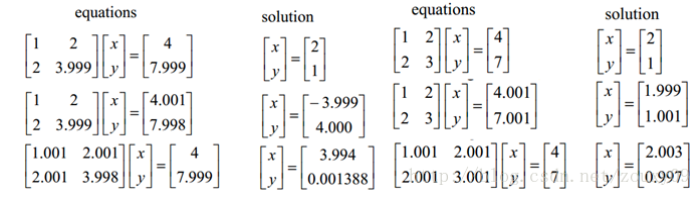
\includegraphics[width=6in]{img/3-1.png}
	\caption{ill-condition}\label{fig:3-1}
	\end{figure}
	
	第一行我们假设$Ax=b$,第二行我们稍微改变下$A$,结果的变化就非常大,第三行我们稍微改变下$b$,结果的改变同样是非常大的,因此我们可以认为我们的模型对错误的容忍力太低了,即对误差太敏感了。那么对于数据中难免存在的误差来说,模型的效果就非常差。
	
	因此我们需要一个指标去衡量ill-condition问题中的变化问题。
	
	condition number 衡量的就是在输入发生微小改变的时候,输出会发生多大的变化。也就是对系统微小变化的敏感度。condition number比较小(在1附近)的就是well-condition的,比较大的(远大于1的)就是ill-condition的。
	
	另外如果使用迭代优化的算法,当condition number太大的时候,会拖慢迭代的收敛速度。
	
	\subsection{L1}
	L1 norm 就是绝对值的和,公式如下
	
	$\|x\|_p = |x_1|+|x_2|+...+|x_n|$
	
	L1可以用来产生稀疏解,即参数具有0的最优值
	
	\subsection{L2}
	L2 norm 就是我们经常说的欧几里得范数,公式如下
	
	\begin{equation}
		\|x\|_2 = (\sum_{i=1:n}x_i ^{2})^{\frac{1}{2}}
	\end{equation}
	
	使用了L2 norm 后一个模型具有以下总的目标函数
	
	\begin{equation}
		\hat{J}(w;X,y) = \frac{\lambda}{2}\omega^T \omega +J(w;X,y)
	\end{equation}
	
	但是需要注意的是,由于$\omega^T \omega$与b无关,因此加入正则化项后,对于b的更新是没有任何影响的
	
	
	caffe中weight decay 这个参数代表L2范数前的系数。
	
	L2的优点:
	\begin{itemize}
		\item 可以防止过拟合,提升模型的泛化能力
		\item L2范数有助于处理condition number不好的情况下逆矩阵求逆很困难的情况(待定)。
	\end{itemize}

	
	
	\subsection{L1与L2的不同}
	对于L1和L2规则化的代价函数来说,我们可以写成如下的形式
	
	\begin{equation}
		Lasso:\min_{w} \frac{1}{n} \|y-Xw\|^2,s.t.\|w\|_1<=C
	\end{equation}
	
	\begin{equation}
		Ridge:\min_{w} \frac{1}{n} \|y-Xw\|^2,s.t.\|w\|_2<=C
	\end{equation}
	
	为了便于可视化,我们考虑两维的情况,在$(w_1,w_2)$平面上画出目标函数的等高线,而约束条件则成为平面上半径为C的一个norm ball。等高线与norm ball相交的地方就是最优解:
	
	\begin{figure}[htbp]
	\centering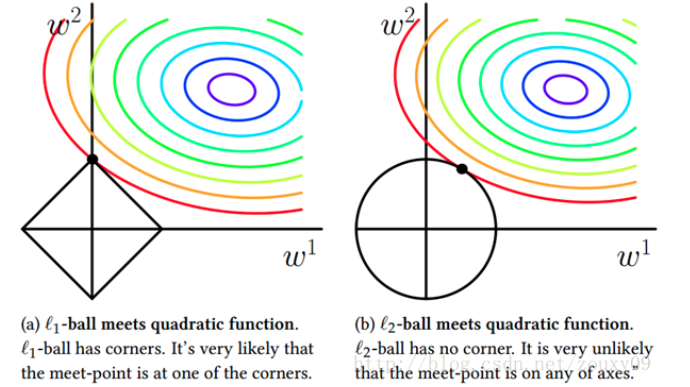
\includegraphics[width=6in]{img/3-2.png}
	\caption{图}\label{fig:3-2}
	\end{figure}
	
	可以看到,在相交的地方,L1在和每个坐标轴相交的地方都有出现解,即更容易出现$w_1$或者$w_2$为0的解,可以用来提取特征,更加容易产生稀疏性。
	
	L2的话更容易出现$w_1$和$w_2$都不是0的情况,虽然有时候会出现很小的值。在更高维的情况下也是这样的,即基本上只是用来正则化而已。
	



\section{数据集增强}

	需要注意的问题
	\begin{itemize}
		\item 不能应用改变正确类别的转换,如:光学字符识别任务需要认识到'b'和'd'的区别,因此对于这种任务来说,水平反转和旋转180度并不是适当的数据集增强方式。
		\item 在神经网络的输入层加入噪声,也可以看成是数据增强的一种形式。然而,神经网络被证明对噪声不是非常健壮。改善神经网络健壮性的方法之一是简单的将随机噪声施加到输入再进行训练。像隐藏单元事假噪声也是可行的,这被看成是在多个抽象层上进行数据集增强。实践证明,噪声被细心调整后,该方法是非常有效的。Dropout可以被看做是通过乘性噪声构建新输入的过程。
		\item 在进行数据集增强的时候,需要进行对照试验。
		
	\end{itemize}
	

\section{提前终止}
	有时候会出现,虽然训练集的误差随着时间的推移逐渐降低,但是训练集的误差再次上升的情况。这种情况下我们需要提前终止模型的训练过程。
	
	提前终止可以单独使用或与其它的正则化策略相结合。
	
	提前终止需要验证集,即这一部分数据相当于在我们的训练过程中是没有参与模型的训练的。我们有两种策略来更好的使用所有的数据。第一种是,第一次训练我们使用训练数据确定最佳的训练步数,然后重新初始化网络,使用所有的数据进行训练。第二种是我们保持从第一轮训练获得的参数,然后使用所有的数据进行训练,但是这样的话,已经没有验证集可以指导我们需要在多少步后进行终止。	
	
\section{参数共享}
	参数共享也是一种正则化方法,是指强迫某些集合中的参数相等。
	
	优点:可以显著减少模型所占用的内存
	
	比如:卷积神经网络
	
\section{bagging}
	Bagging:是通过结合几个模型降低泛化误差的技术。即分别训练几个不同的模型,让所有模型表决测试样例的输出。
	
	Bagging奏效的原因:不同的模型通常不会在测试集上产生完全相同的错误。
	
	假设有k个不同的模型。在不同模型的误差完全相关的情况下,bagging对于降低泛化误差没有任何帮助。但是在模型误差完全不相关的情况下,bagging后的误差仅为之前误差的$\fr\frac{1}{k}$(期望)。这表明,模型的个数越多,则集成模型的误差降低的越小,呈线性关系,即集成后的模型最起码表现的比它的任何一个成员都要好。如果成员之间的误差是独立的,则集成将显著地比其成员表现得更好。
	
	Bagging需要构造k个不同的数据集,每个数据集与原始数据集具有相同数量的样例,但从原始样例中替换采样构成。即新的数据集中包含若干重复的实例,还会缺少很多实例。每个数据集包含样本的差异将导致训练模型之间的差异。
	

\section{Dropout}
	Dropout可以看成是集成非常多的大神经网络的Bagging方法。但是在Dropout中不同的模型之间是共享参数的,也就是说不同的模型之间具有相同的神经元的数量,但是在每一层中的神经元的个数可能是不同的,这一层中使用哪一个神经元也是不同的。
	
	在使用Dropout时,每次训练的过程都只是一个子网络在训练,而不是训练整个网络。这也意味着,在一些小型的神经网路中使用Dropout并不是一个非常好的选择,而应该在一个大型的网络中使用Dropout。也就是说,使用Dropout的代价就是提高了模型的计算代价。需要注意的是,如果你有非常大的训练数据集,使用Dropout进行正则化带来的好处可能小于所带来的计算代价的提升。
	
	同样,在只有极少(如小于5000个)的训练样本可用时,Dropout不会很有效。
	
	Dropout强大的大部分是由于施加到隐藏单元的乘性掩码噪声。BN是在训练时向隐藏单元引入加性和乘性造成,同时这个噪声具有正则化的效果,有时候Dropout变得没有必要。
	
	需要注意的是,在有些深度学习框架中,dropout ratio表示的是保留的神经元的比例,有些是丢弃的神经元的比例。但是在大多数的神经网络的框架中都是表示保留的神经元的比例。
	
\section{Spatial Dropout}
	
	如图所示,对于一个特征来说,传统的Dropout在随机丢弃点的时候,会丢弃这个特征中的一些点。而Spatial Dropout会直接丢弃整个特征。在实际的应用中,如在做物体检测,或者使用Unet的过程中Spatial Dropout的表现是更好的。
	\begin{figure}[!htbp]
	\centering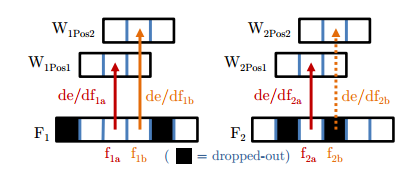
\includegraphics[width=6in]{img/3-3.png}
	\caption{原始Dropout}\label{fig:3-3}
	\end{figure}
	\newpage
	
	\begin{figure}[!htbp]
	\centering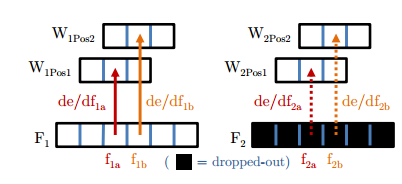
\includegraphics[width=6in]{img/3-4.png}
	\caption{Spatial Dropout}\label{fig:3-4}
	\end{figure}

\section{对抗训练}

	\begin{figure}[!htbp]
	\centering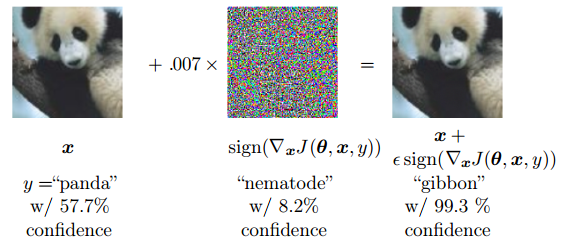
\includegraphics[width=6in]{img/3-5.png}
	\caption{图}\label{fig:3-5}
	\end{figure}
	
	通过添加一个不可察觉的小向量,我们可以改变GoogleNet对此图像的分类结果。如上图所示,我们人类可能不能观察出这种区别,但是网络的预测结果可能会千差万别。
	
	对于上述这种情况我们可能需要使用对抗训练来进行正则化。
	
	但是具体对抗训练是什么样的,暂时不清楚。---待补充
	
	
	
	
	
	
	
	
	
	
	
	
	
	
	
	
	
	
	
	
	
	